\section{Lernen im Unternehmen}

\frame{\titlepage}

\frame{
  \frametitle{Agenda}

  \tableofcontents
}

\frame{
  \frametitle{Was bedeutet ,,lernen''?}

  Was bedeutet ,,lernen''?

  \begin{itemize}
    \item Aristoteles ca. 350 v.Chr.: Wahrnehmung führt zu einer Kopie der Objekte im Geist, die wir irgendwann ,,kennen'' \cite{Lefrancois:2006}
    \item Strenggenommen: (Er-)Kenntnis. Aber der Weg zur Erkenntnis: Wahrnehmung (vgl. Konstruktivismus \cite{Watzlawick:1992})
      % Wahrnehmung kann sehr selektiv sein (wie wir bei Herrn Huebner gelernt haben)
    \item Definition: Dauerhafte Veränderungen im Verhaltenspotential, die aus Erfahrung resultieren, aber nicht durch Müdigkeit, Reifung, Drogengebrauch, Verletzung oder Krankheit verursacht sind \cite{Lefrancois:2006}
  \end{itemize}
}

\subsection{Motivation und Problematik}

\frame{
  \frametitle{Motivation: Worum geht es?}

  \vspace{-0.2cm}

  \begin{columns}
    \column{0.78\textwidth}
      Laut S. Franken \cite{Franken:2007} geht es dabei darum:

      \begin{itemize}
        \item basierend auf individuellem und Gruppenlernen
        \item Lernprozesse der Mitarbeiter zu initiieren und zu steuern
      \end{itemize}

    \column{0.22\textwidth}
      
\includegraphics[width=1\textwidth]{images/learning-company.png}
  \end{columns}

  Erfordert ausserdem:

  \begin{itemize}
    \item Aktives Auseinandersetzen mit der Unternehmensumwelt
    \item Individuell und selbstorganisiert
    \item Betriebsspezifische Variiationen
  \end{itemize}

  \vspace{0.2cm}

  $\rightarrow$ Individuelles Lernen \\
  \hspace{0.1cm} $\rightarrow$ Austausch, Interaktion, Harmonisierung \\
  \hspace{0.2cm} $\rightarrow$ Gruppenlernen
}

\frame{
  \frametitle{Herausforderungen 1}

  \begin{columns}
    \column{0.5\textwidth}
      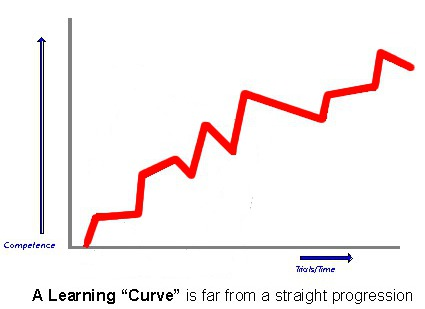
\includegraphics[width=1\textwidth]{images/learning-curve.jpg} \cite{curve1}

    \column{0.5\textwidth}
      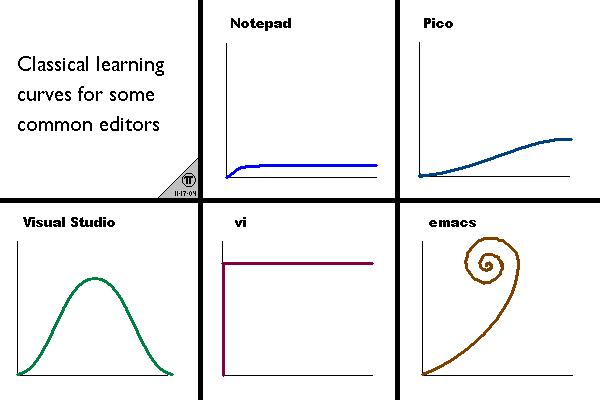
\includegraphics[width=0.9\textwidth]{images/curves.jpg} \cite{curve2}
      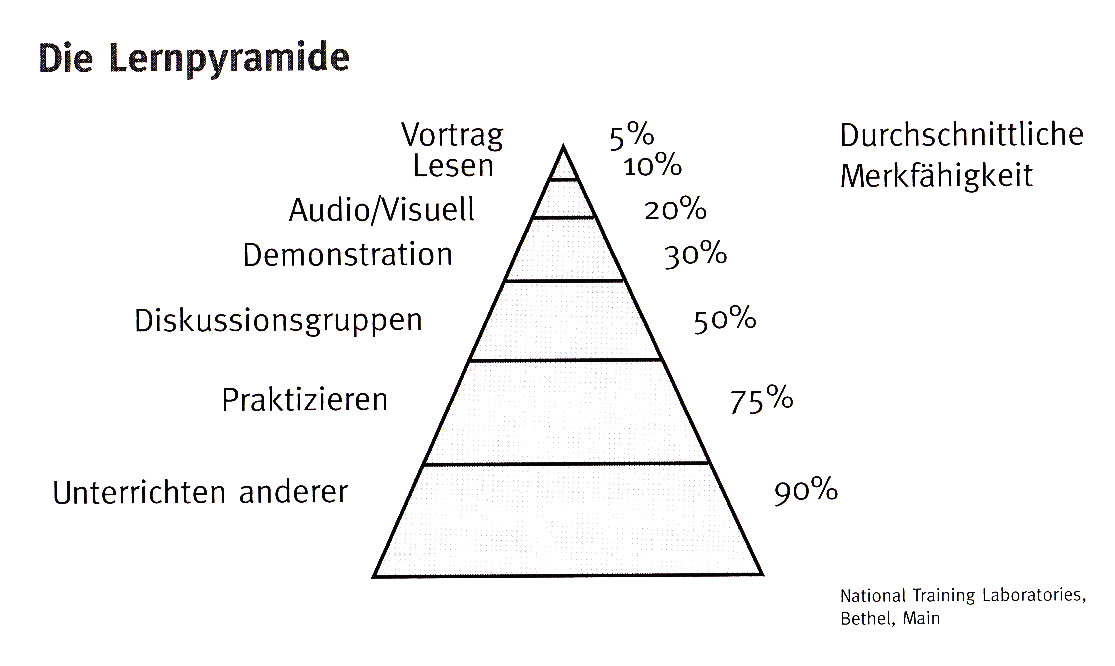
\includegraphics[width=1\textwidth]{images/lernpyramide.jpg} \cite{pyramid}
  \end{columns}

  % Eine Lernkurve ist idR. nicht immer gradlinig und progressiv, was das Lernen im Unternehmen
  % als Management-Aufgabe, die Planung erfordert so schwierig macht

  % Positive unternehmerische Auswirkungen organisationalen Lernens ggf. stark zeitversetzt
}

\frame{
  \frametitle{Herausforderungen 2}

  ,,We might already be beyond the age of speed, by moving into the age of real-time.''
  - Ivan Illich, Austrian philosopher (1926-2002)

  \vspace{0.25cm}

  Nur ein lernfähiges Unternehmen kann in einer Wissensgesellschaft erfolgreich
  sein. \cite{Franken:2007}

  \vspace{0.25cm}

  \begin{columns}
    \column{0.6\textwidth}
      Weitere Herausforderungen:

      \begin{itemize}
        \item Informationsflut (Zeit, Geld, Komplexität)
        \item Gruppenverhalten und -Rollen \cite{Huebner:2011}
        \item Kommunikationsprobleme \cite{Huebner:2011}
          % Verschiedene Erwartungen, potentielle Konflikte, unterschiedliche Wahrnehmung (Konstruktivismus)
        \item selektive Wahrnehmung \cite{Huebner:2011}
          % Bevorzugte Wahrnehmung dessen was, ich wahrnehmen will und erwarte
        \item ...
      \end{itemize}

    \column{0.4\textwidth}
      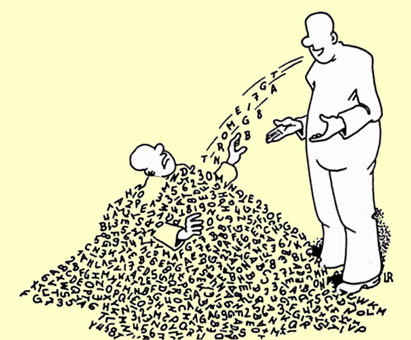
\includegraphics[width=1\textwidth]{images/Informationsflut.jpg} \cite{flood}
  \end{columns}
}

\frame{
  \frametitle{Das Unternehmen als Individuum}

  Das Unternehmen als Individuum, sich selbst organisierende und gestaltende
  soziale Handlungseinheit

  \begin{itemize}
    % Möglich, aufgrund langfristiger Erreichung gemeinsamer Ziele
    \item Analogie um Lernprozesse im Unternehmen besser nachzuvollziehen
    \item Unternehmskultur entspricht der Persönlichkeit
    \item Das unternehmerische Handeln ist das bewusste Tun
    % wodurch es sich selbst oder seine Umwelt verändert
  \end{itemize}

  Lernprozess im Unternehmen nach P. Pawlowsky \cite{Pawlowsky:1992}:

  \begin{itemize}
    \item Die Wissensbasis bestimmt das Handeln
    \item Interaktion mit interner und externer Umwelt
    \item Die Konsequenzen initiieren den Lernprozess
    \item Der Lernprozess verändert die Wissensbasis
  \end{itemize}

  \begin{block}{Resultat}
    Bessere Systemanpassung und Problemlösungsfähigkeit
  \end{block}

  % Beispiel
}

\frame{
  \frametitle{Organisationale Wissensbasis}

  \begin{columns}
    \column{0.7\textwidth}
      Organisationale Wissensbasis:

      \begin{itemize}
        \item Bildet sich durch kollektives Lernen des Systems
        \item Individuelles Lernen reicht nicht
      \end{itemize}

    \column{0.3\textwidth}
      
\includegraphics[width=1\textwidth]{images/buecher.jpg}
  \end{columns}

  \vspace{0.5cm}

  H. Wilke \cite{Wilke:2001}: Das organisationale Lernen hat erst (vollständig) stattgefunden, wenn
  Veränderungen der Regelsysteme des Systems erkennbar werden und wirksam sind.
}

\subsection{Organisationale Lerntheorien}

\frame{
  \frametitle{Cyert und March}

  Cyert und March \cite{Cyert:1992} in den 50-60er Jahren:

  \begin{itemize}
    \item Vorher: Unternehmen als rationales, über alle notwendigen Informationen verfügendes System
    \item Cyert und March: Unternehmen als adaptives, sich anpassendes rationales System
          % potentiell verschiedene Systemzustände
          % effektiv realisierter Zustand durch Umwelteinflüsse und eigene Ziele gesteuertes Verhalten bestimmt
  \end{itemize}

  \begin{columns}
    \column{0.5\textwidth}
      Grundlegene Prinzipien:
      % bzgl. der Anpassung

      \begin{itemize}
        \item Vermeide Unsicherheit
        \item Halte an bewährten Regelsystemen fest
        \item Benutze einfache Regeln
      \end{itemize}

      % Verhalten wird durch vier Hauptkonzepte bestimmt
      % - Quasilösung von Konflikten
      % - Vermeidung von Ungewissheit
      % - Problemorientierte Suche
      % - Organisatorisches Lernen

    \column{0.5\textwidth}
      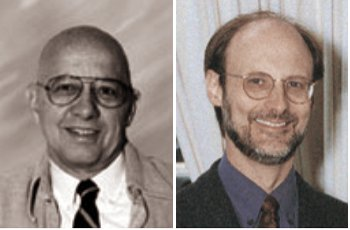
\includegraphics[width=0.8\textwidth]{images/cyert_march.jpg}
  \end{columns}
}

\frame{
  \frametitle{Kritik bzgl. Cyert und March}

  \vspace{0.3cm}

  Kritik bzgl. Cyert und March:

  \begin{itemize}
    \item Organisationales Lernen ist mehr als bloßes Anpassen
    \item Passive, ausschließlich reagierende Unternehmen
    \item Lernen primär aus ,,Krisen'' (akute Probleme)
      % Am Anfang steht das "Problem"
      % Lernen einzig aus resultierenden Umweltreaktionen
      % Erinnert an Trial und Error
    \item Lernen in Zyklen
      % Erfahrungsorientiertes Lernen
      % Erfahrung bildet Handlungstheorien -> Handlung -> Konsequenzen -> Diskrepanzen erfordern Anpassung der Theorien
      % Langsam, Reaktiv
  \end{itemize}

  \begin{center}
    
\includegraphics[width=0.5\textwidth]{images/zirkel}
  \end{center}
}

\frame{
  \frametitle{Argyris und Schön}

  Argyris und Schön nach S. Franken \cite{Franken:2007}:

  \begin{itemize}
    \item Unternehm. Handeln als individuelles durch Rollen geleitetes
    \item Geäußerte Handlungstheorien VS reale Gebrauchstheorien
    \item Diskrepanzen initiieren Lernprozesse
      % Entfernt verwandt mit Kognitiver Dissonanz (Huebner), aber es geht nicht primär um Gefühle
    \item Hintergrund: Konstruktivistischer Lernansatz (vgl. \cite{Watzlawick:1992})
    \item Drei Lerntypen: Single-Loop, Double-Loop, Deutero
      % Zielabweichungen werden erkannt und korrigiert
      % Nur Anpassung der Parameter in vorgegebenem Schemata
      % Beispiel: Sinkender Absatz erfordert mehr Werbung und Verkaufsaktivitäten

      % Lernen durch Bewertung und Entwicklung von Schemata
      % Modifikation und Verbesserung der allgemeinen Regeln, Normen und Ziele
      % Quasi: Ursachenanalyse
      % Beispiel: sinkender Absatz führt zur Überprüfung, ob dies an zu wenig Werbung oder mangelnder Produktqualität liegt

      % Lernendes Lernen, höchstes Lernniveau
      % Selbstreflexion der Lernprozesse, mit Wissen aus vergangenen Lernprozessen

    % Wenn Double-Loop oder Deutero Lernen nicht erreicht wird können die Ursachen bspw. in defensivem Verhalten der Miterbeiter liegen
    % und dem Wunsch negative Gefühle zu vermeiden. Probleme werden dann vertuscht und unterdrückt um vor negativen Gefühlen zu schützen.
  \end{itemize}

  % Erfordert offene und konstruktive Lern- und Diskussionskultur

  \begin{columns}
    \column{0.5\textwidth}
      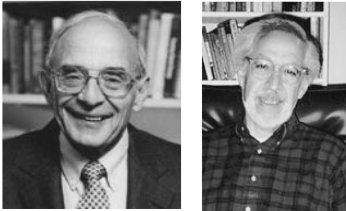
\includegraphics[width=0.8\textwidth]{images/agyris_schoen.jpg}
    \column{0.5\textwidth}
      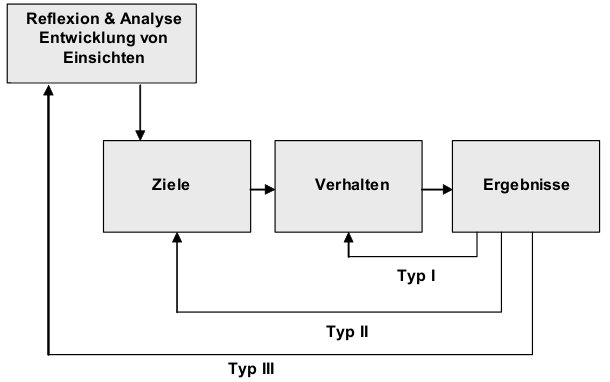
\includegraphics[width=0.95\textwidth]{images/lerntypen.jpg} \cite{Agyris:1999}
  \end{columns}
}

\frame{
  \frametitle{Vorraussetzungen}

  Strukturelle und kulturelle Vorraussetzungen:

  \begin{itemize}
    \item bzgl. der Entscheidungs- und Hierarchieebenenen
    \item Refelexionsfähigkeit für höhere Lernebenen
    \item Offene und konstruktive Lern- und Diskussionskultur
  \end{itemize}

  \begin{center}
    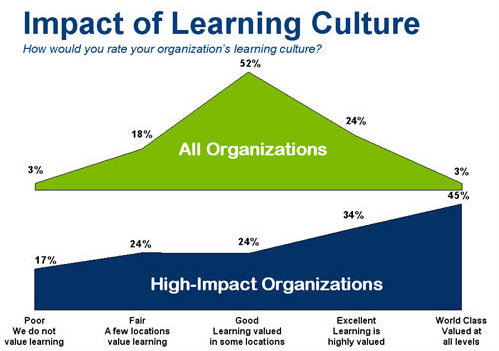
\includegraphics[width=0.65\textwidth]{images/culture.jpg} \cite{culture}
  \end{center}
}

%\frame{
%  \frametitle{P. Senge}
%
%  \begin{columns}
%    \column{0.75\textwidth}
%      \begin{block}{Unternehmen sind}
%        ,,ein Ort, an dem Menschen kontinuierlich entdecken, dass sie ihre Realität
%        selbst erschaffen. Und dass sie sie verändern können.''
%      \end{block}
%
%    \column{0.2\textwidth}
%      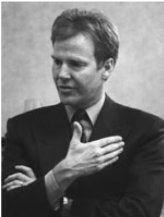
\includegraphics[width=1\textwidth]{images/senge.jpg}
%  \end{columns}
%
%  \vspace{0.3cm}
%
%  Sieben Hindernisse bzgl. des Lernens in Unternehmen:
%
%  \vspace{0.3cm}
%
%  \begin{columns}
%    \column{0.55\textwidth}
%      \begin{itemize}
%        \item Ich bin meine Position
%        \item Der Feind da draußen
%        \item Angriff ist die beste Verteidigung
%        \item Fixierung auf Ereignisse
%      \end{itemize}
%
%    \column{0.55\textwidth}
%      \begin{itemize}
%        \item Gleichnis vom gekochten Fisch
%        \item Illusion aus Erfahrung zu lernen
%        \item Mythos vom Managementteam
%      \end{itemize}
%  \end{columns}
%}

%\frame{
%  \frametitle{,,Fünf Disziplinen'' als Lösung}
%
%  \begin{center}
%    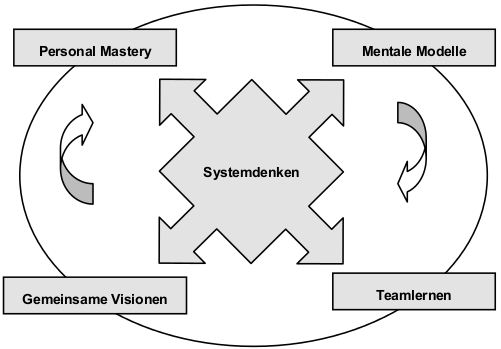
\includegraphics[width=0.8\textwidth]{images/senge.png}
%  \end{center}
%}

\frame{
  \frametitle{Das lernende Unternehmen: in Richtung Gegenwart ...}

  \vspace{0.3cm}

  Nonaka und Takeuchi:

  \begin{itemize}
    \item Schaffung neuen Wissens steht über Wissensverarbeitung
    \item Ständige Erneuerung der Denk- und Handlungsmodelle
    \item Lerndimensionen im Unternehmen:
    \begin{itemize}
      \item Epistemologische Dimension: explizites und implizites Wissen
        % explizit: dokumentiertes Wissen
        % implizit: Wissen in den Köpfen
      \item Ontologische Dimension: Individuum und Kollektiv
    \end{itemize}
  \end{itemize}

  Nur Einzelpersonen erzeugen Wissen. Das Unternehmen muss deren Kreativität
  unterstützen, und im Wissensnetz verankern.
}

\frame{
  \frametitle{Nonaka und Takeuchi: die vier Dimensionen}

  \begin{center}
    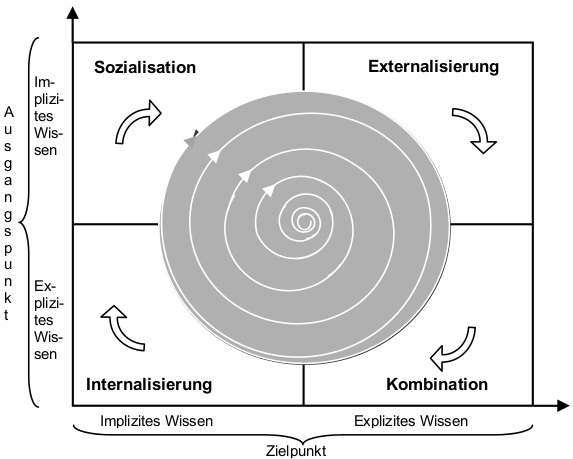
\includegraphics[width=0.75\textwidth]{images/nonaka.png}
  \end{center}

  % Sozialisation:
  % Wandelt implizites Wissen wird durch Austausch bei Beobachtung und Nachahmung in explizites Wissen umgewandelt

  % Internalisierung:
  % Wandelt explizites Wissen in implizites Wissen um. Beispiel: Film über die Firmenphilosophie vermittelt explizites Wissen

  % Externalisierung:
  % Implizites Wissen wird in Form expliziter Aussagen oder Fakten kommunizierbar gemacht.

  % Kombination:
  % Verschiedene Bereiche expliziten Wissens werden kombiniert und bspw. über Medien und Dokumente ausgetauscht.

  % Verschiedene Phasen der Wissensgewinnung:
  % - Wissen austauschen
  % - Konzepte schaffen
  % - Konzepte erklären
  % - Einen Archetyp bilden
  % - Wissen übertragen

  % Verschiedene Vorraussetzungen:
  % - Intention
  % - Autonomie
  % - Redundanz
  % - Fluktuation und kreatives Chaos
  % - Notwendige Vielfalt
}

\subsection{Gegenwart/Zunkunft des lernenden Unternehmens}

\frame{
  \frametitle{Das lernende Unternehmen: Gegenwart/Zukunft}

  \begin{alertblock}{Kritik}
    Die Theorien berücksichtigen IMHO die digitale Informationsgesellschaft und Globalisierung nicht ausreichend
  \end{alertblock}

  \begin{itemize}
    \item Individuen sind nicht ,,isoliert''
      % Das soll nicht heissen dass die vorgestellten Theorien von isolierten Unternehmen ausgehen
      % aber Auswirkungen des Internets werden bspw. nicht ausreichend berücksichtigt
    \item Ständiger Zugriff auf unterschiedliche Netzwerke möglich
    \item Unternehmensumwelt kaum mehr überschaubar und dynamisch
  \end{itemize}
}

\frame{
  \frametitle{Konnektivismus}

  \begin{columns}
    \column{0.75\textwidth}
      Konnektivismus nach G. Siemens \cite{Siemens:2005}:

      \begin{itemize}
        \item Der Mensch als vernetzte Entität
        \item Zugriff auf andere menschliche und technische Netze
      \end{itemize}

    \column{0.25\textwidth}
      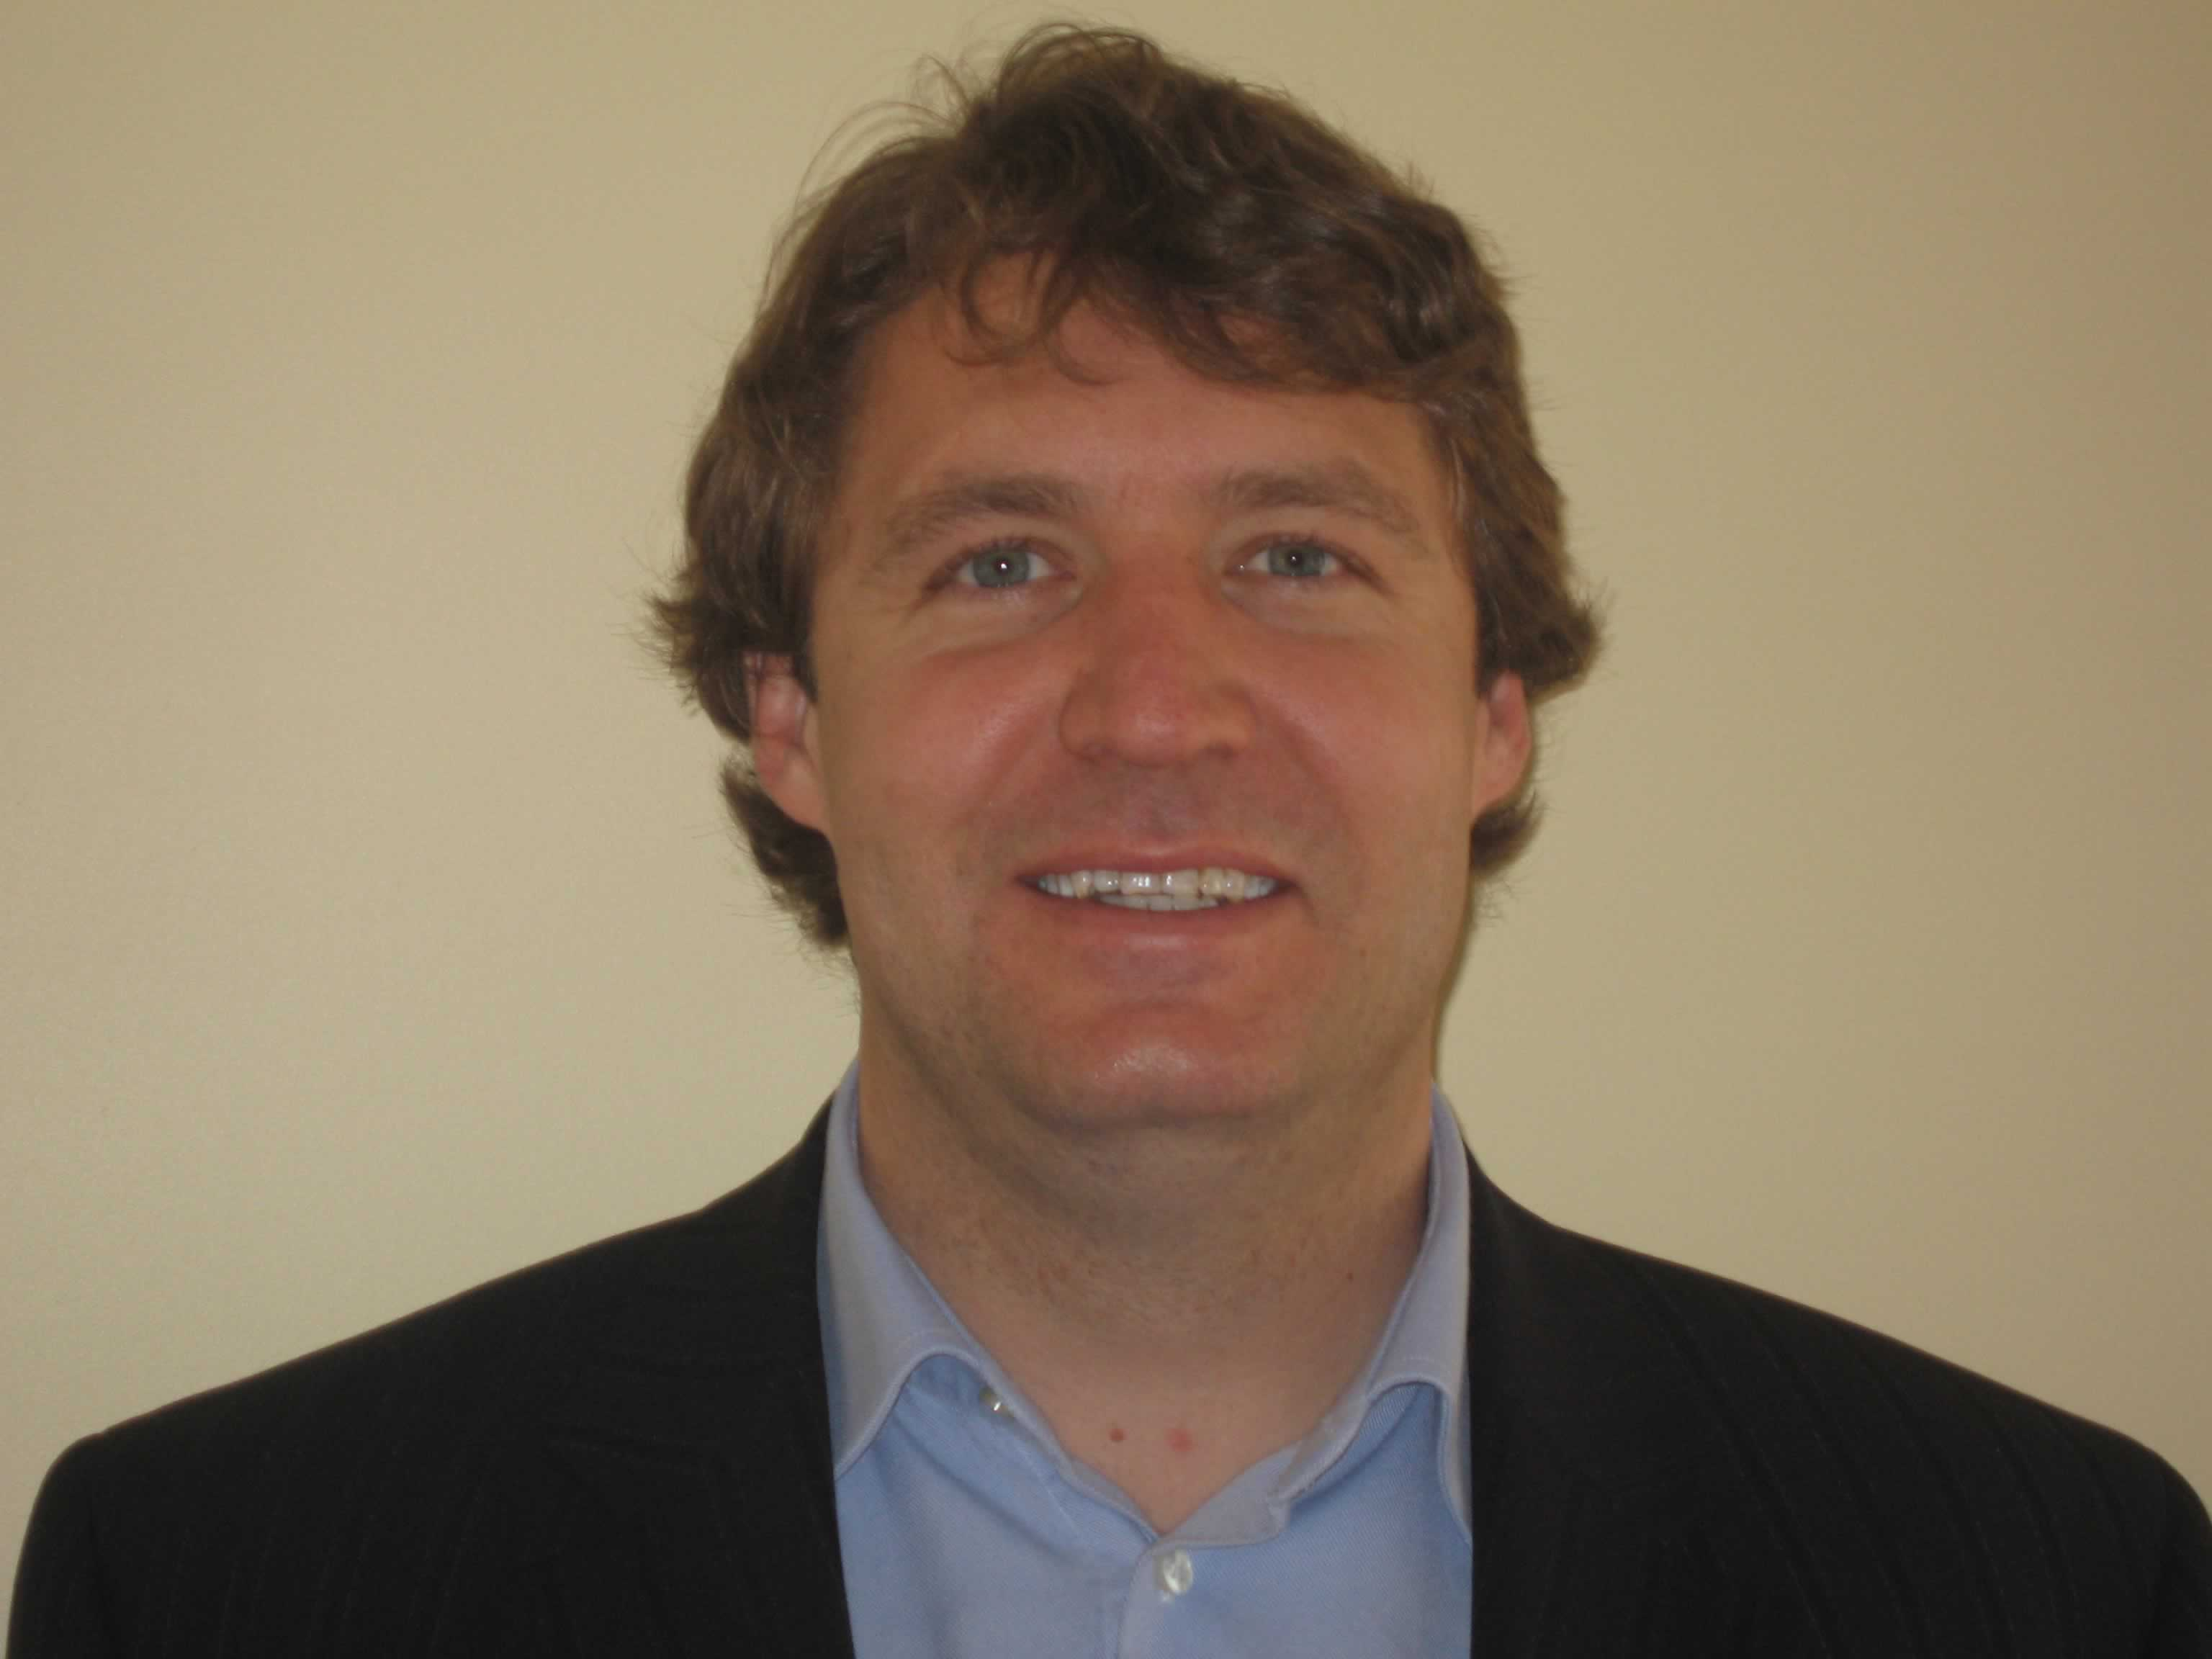
\includegraphics[width=1\textwidth]{images/gsiemens.jpg}
  \end{columns}

  \vspace{0.3cm}

  Zentrale Annahmen:

  \begin{itemize}
    \item Vernetzung über ,,Knoten und Verbindungen''. Knoten sind bspw. Menschen, Internetseiten, Bücher, Grafiken, etc.
    \item Schaffen neuer Verbindungen zu Knoten = Lernen
    \item ,,Wissen: Wo'' ebenso wichtig wie das ,,Wissen: Wie/Wo''
  \end{itemize}

  \textbf{Kritik}: Konnektivismus ist im Grunde keine Lerntheorie, sondern eine pädagogische Sichtweise \cite{Verhagen:2006}
}

\subsection{Zusammenfassung}

\frame{
  \frametitle{Zusammenfassung}
}


